\section{Construction of the parser}
	In this section we will describe how one can construct a parser from a EBNF, but first we will describe how a parser is and how it works.
	
	\subsection{Parsing strategies}
		The job of a parser is to check if a program is correct and 
		to determine the structure of the program, usually done by constructing a tree structure.
		There are two common ways of checking this {\it Bottom-up Parsing} and {\it Top-Down Parsing}.
		
		\subsubsection*{Bottom-up Parsing}
			This way of parsing takes simple structures and combining them to more complex structures.
			We call this type of parsing for {\it LR parsing} because we read the text from the left and reduces to the right.
			\begin{figure}[H]
				\centering
				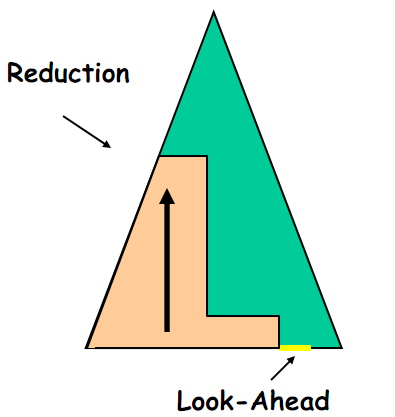
\includegraphics[width=0.5\textwidth]{rapport/2/figures/bottomup.png}
				\caption{LR Parsing}\label{fig:lrparse}
			\end{figure}
			
		\subsubsection*{Top-down Parsing}
			Top-down parsing starts from the complex structures are breaks them down into smaller parts.
			We call this type of parsing for {\it LL parsing} because we read the text from the left and make derivations to the left.
			\begin{figure}[H]
				\centering
				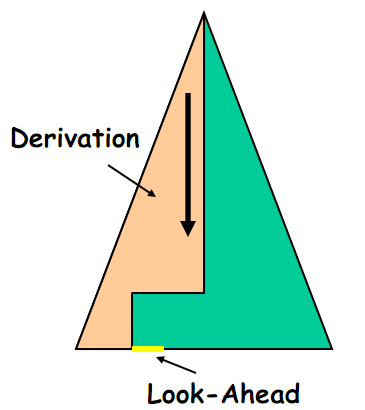
\includegraphics[width=0.5\textwidth]{rapport/2/figures/topdown.png}
				\caption{LL Parsing}\label{fig:llparsing}
			\end{figure}
	
	\subsection{Creating a recursive descent parser}
		A recursive descent parser is a LL parser which works by recursively going through the program.
		To construct this type of parser a EBNF is required and here is how it is made:
		\begin{enumerate}
			\item Make a scanner for reading chars and identifying them as terminals.
			\item Make a parse method for each non-terminal in the EBNF.
			\item Make a method that can accept terminals.
			\item In each of the parse method accept terminals and/or call other parse methods.
		\end{enumerate}		
		
		
		
		